\documentclass[10pt,a4paper]{article}
\usepackage{tikz}
\usetikzlibrary{matrix,calc}
\usepackage{multirow}
\usepackage[utf8]{inputenc}
\usepackage[spanish]{babel}
\usepackage{amsmath}
\usepackage{amsfonts}
\usepackage{amssymb}
\usepackage{graphicx}
\usepackage{float}
\usepackage[left=2cm,right=2cm,top=2cm,bottom=2cm]{geometry}
\usepackage{circuitikz}
\usepackage{tikz-timing}
\usetikztiminglibrary[rising arrows]{clockarrows}
\usepackage{pgfplots}
\pgfplotsset{compat=1.15}
\usepackage{listings}
\usepackage[export]{adjustbox}
\usepackage{graphicx,wrapfig,lipsum}
\usepackage{booktabs}
\usepackage[skip=0pt]{caption}
\captionsetup[figure]{font=small,labelfont=small}


\usetikzlibrary{matrix,calc}

%isolated term
%#1 - Optional. Space between node and grouping line. Default=0
%#2 - node
%#3 - filling color
\newcommand{\implicantsol}[3][0]{
    \draw[rounded corners=3pt, fill=#3, opacity=0.3] ($(#2.north west)+(135:#1)$) rectangle ($(#2.south east)+(-45:#1)$);
    }


%internal group
%#1 - Optional. Space between node and grouping line. Default=0
%#2 - top left node
%#3 - bottom right node
%#4 - filling color
\newcommand{\implicant}[4][0]{
    \draw[rounded corners=3pt, fill=#4, opacity=0.3] ($(#2.north west)+(135:#1)$) rectangle ($(#3.south east)+(-45:#1)$);
    }

%group lateral borders
%#1 - Optional. Space between node and grouping line. Default=0
%#2 - top left node
%#3 - bottom right node
%#4 - filling color
\newcommand{\implicantcostats}[4][0]{
    \draw[rounded corners=3pt, fill=#4, opacity=0.3] ($(rf.east |- #2.north)+(90:#1)$)-| ($(#2.east)+(0:#1)$) |- ($(rf.east |- #3.south)+(-90:#1)$);
    \draw[rounded corners=3pt, fill=#4, opacity=0.3] ($(cf.west |- #2.north)+(90:#1)$) -| ($(#3.west)+(180:#1)$) |- ($(cf.west |- #3.south)+(-90:#1)$);
}

%group top-bottom borders
%#1 - Optional. Space between node and grouping line. Default=0
%#2 - top left node
%#3 - bottom right node
%#4 - filling color
\newcommand{\implicantdaltbaix}[4][0]{
    \draw[rounded corners=3pt, fill=#4, opacity=0.3] ($(cf.south -| #2.west)+(180:#1)$) |- ($(#2.south)+(-90:#1)$) -| ($(cf.south -| #3.east)+(0:#1)$);
    \draw[rounded corners=3pt, fill=#4, opacity=0.3] ($(rf.north -| #2.west)+(180:#1)$) |- ($(#3.north)+(90:#1)$) -| ($(rf.north -| #3.east)+(0:#1)$);
}

%group corners
%#1 - Optional. Space between node and grouping line. Default=0
%#2 - filling color
\newcommand{\implicantcantons}[2][0]{
    \draw[rounded corners=3pt, opacity=.3] ($(rf.east |- 0.south)+(-90:#1)$) -| ($(0.east |- cf.south)+(0:#1)$);
    \draw[rounded corners=3pt, opacity=.3] ($(rf.east |- 8.north)+(90:#1)$) -| ($(8.east |- rf.north)+(0:#1)$);
    \draw[rounded corners=3pt, opacity=.3] ($(cf.west |- 2.south)+(-90:#1)$) -| ($(2.west |- cf.south)+(180:#1)$);
    \draw[rounded corners=3pt, opacity=.3] ($(cf.west |- 10.north)+(90:#1)$) -| ($(10.west |- rf.north)+(180:#1)$);
    \fill[rounded corners=3pt, fill=#2, opacity=.3] ($(rf.east |- 0.south)+(-90:#1)$) -|  ($(0.east |- cf.south)+(0:#1)$) [sharp corners] ($(rf.east |- 0.south)+(-90:#1)$) |-  ($(0.east |- cf.south)+(0:#1)$) ;
    \fill[rounded corners=3pt, fill=#2, opacity=.3] ($(rf.east |- 8.north)+(90:#1)$) -| ($(8.east |- rf.north)+(0:#1)$) [sharp corners] ($(rf.east |- 8.north)+(90:#1)$) |- ($(8.east |- rf.north)+(0:#1)$) ;
    \fill[rounded corners=3pt, fill=#2, opacity=.3] ($(cf.west |- 2.south)+(-90:#1)$) -| ($(2.west |- cf.south)+(180:#1)$) [sharp corners]($(cf.west |- 2.south)+(-90:#1)$) |- ($(2.west |- cf.south)+(180:#1)$) ;
    \fill[rounded corners=3pt, fill=#2, opacity=.3] ($(cf.west |- 10.north)+(90:#1)$) -| ($(10.west |- rf.north)+(180:#1)$) [sharp corners] ($(cf.west |- 10.north)+(90:#1)$) |- ($(10.west |- rf.north)+(180:#1)$) ;
}

%Empty Karnaugh map 4x4
\newenvironment{Karnaugh}%
{
\begin{tikzpicture}[baseline=(current bounding box.north),scale=0.8]
\draw (0,0) grid (4,4);
\draw (0,4) -- node [pos=0.7,above right,anchor=south west] {cd} node [pos=0.7,below left,anchor=north east] {ab} ++(135:1);
%
\matrix (mapa) [matrix of nodes,
        column sep={0.8cm,between origins},
        row sep={0.8cm,between origins},
        every node/.style={minimum size=0.3mm},
        anchor=8.center,
        ampersand replacement=\&] at (0.5,0.5)
{
                       \& |(c00)| 00         \& |(c01)| 01         \& |(c11)| 11         \& |(c10)| 10         \& |(cf)| \phantom{00} \\
|(r00)| 00             \& |(0)|  \phantom{0} \& |(1)|  \phantom{0} \& |(3)|  \phantom{0} \& |(2)|  \phantom{0} \&                     \\
|(r01)| 01             \& |(4)|  \phantom{0} \& |(5)|  \phantom{0} \& |(7)|  \phantom{0} \& |(6)|  \phantom{0} \&                     \\
|(r11)| 11             \& |(12)| \phantom{0} \& |(13)| \phantom{0} \& |(15)| \phantom{0} \& |(14)| \phantom{0} \&                     \\
|(r10)| 10             \& |(8)|  \phantom{0} \& |(9)|  \phantom{0} \& |(11)| \phantom{0} \& |(10)| \phantom{0} \&                     \\
|(rf) | \phantom{00}   \&                    \&                    \&                    \&                    \&                     \\
};
}%
{
\end{tikzpicture}
}

%Empty Karnaugh map 2x4
\newenvironment{Karnaughvuit}%
{
\begin{tikzpicture}[baseline=(current bounding box.north),scale=0.8]
\draw (0,0) grid (4,2);
\draw (0,2) -- node [pos=0.7,above right,anchor=south west] {bc} node [pos=0.7,below left,anchor=north east] {a} ++(135:1);
%
\matrix (mapa) [matrix of nodes,
        column sep={0.8cm,between origins},
        row sep={0.8cm,between origins},
        every node/.style={minimum size=0.3mm},
        anchor=4.center,
        ampersand replacement=\&] at (0.5,0.5)
{
                      \& |(c00)| 00         \& |(c01)| 01         \& |(c11)| 11         \& |(c10)| 10         \& |(cf)| \phantom{00} \\
|(r00)| 0             \& |(0)|  \phantom{0} \& |(1)|  \phantom{0} \& |(3)|  \phantom{0} \& |(2)|  \phantom{0} \&                     \\
|(r01)| 1             \& |(4)|  \phantom{0} \& |(5)|  \phantom{0} \& |(7)|  \phantom{0} \& |(6)|  \phantom{0} \&                     \\
|(rf) | \phantom{00}  \&                    \&                    \&                    \&                    \&                     \\
};
}%
{
\end{tikzpicture}
}

%Empty Karnaugh map 2x2
\newenvironment{Karnaughquatre}%
{
\begin{tikzpicture}[baseline=(current bounding box.north),scale=0.8]
\draw (0,0) grid (2,2);
\draw (0,2) -- node [pos=0.7,above right,anchor=south west] {b} node [pos=0.7,below left,anchor=north east] {a} ++(135:1);
%
\matrix (mapa) [matrix of nodes,
        column sep={0.8cm,between origins},
        row sep={0.8cm,between origins},
        every node/.style={minimum size=0.3mm},
        anchor=2.center,
        ampersand replacement=\&] at (0.5,0.5)
{
          \& |(c00)| 0          \& |(c01)| 1  \\
|(r00)| 0 \& |(0)|  \phantom{0} \& |(1)|  \phantom{0} \\
|(r01)| 1 \& |(2)|  \phantom{0} \& |(3)|  \phantom{0} \\
};
}%
{
\end{tikzpicture}
}

%Defines 8 or 16 values (0,1,X)
\newcommand{\contingut}[1]{%
\foreach \x [count=\xi from 0]  in {#1}
     \path (\xi) node {\x};
}

%Places 1 in listed positions
\newcommand{\minterms}[1]{%
    \foreach \x in {#1}
        \path (\x) node {1};
}

%Places 0 in listed positions
\newcommand{\maxterms}[1]{%
    \foreach \x in {#1}
        \path (\x) node {0};
}

%Places X in listed positions
\newcommand{\indeterminats}[1]{%
    \foreach \x in {#1}
        \path (\x) node {X};
}
\newenvironment{KarnaughTP3}%
{
\begin{tikzpicture}[baseline=(current bounding box.north),scale=0.8]
\draw (0,0) grid (4,4);
\draw (0,4) -- node [pos=0.9,above right,anchor=south west] {$Q_1 Q_0$} node [pos=0.7,below left,anchor=north east] {$W Q_2$} ++(135:1);
%
\matrix (mapa) [matrix of nodes,
        column sep={0.8cm,between origins},
        row sep={0.8cm,between origins},
        every node/.style={minimum size=0.3mm},
        anchor=8.center,
        ampersand replacement=\&] at (0.5,0.5)
{
                       \& |(c00)| 00         \& |(c01)| 01         \& |(c11)| 11         \& |(c10)| 10         \& |(cf)| \phantom{00} \\
|(r00)| 00             \& |(0)|  \phantom{0} \& |(1)|  \phantom{0} \& |(3)|  \phantom{0} \& |(2)|  \phantom{0} \&                     \\
|(r01)| 01             \& |(4)|  \phantom{0} \& |(5)|  \phantom{0} \& |(7)|  \phantom{0} \& |(6)|  \phantom{0} \&                     \\
|(r11)| 11             \& |(12)| \phantom{0} \& |(13)| \phantom{0} \& |(15)| \phantom{0} \& |(14)| \phantom{0} \&                     \\
|(r10)| 10             \& |(8)|  \phantom{0} \& |(9)|  \phantom{0} \& |(11)| \phantom{0} \& |(10)| \phantom{0} \&                     \\
|(rf) | \phantom{00}   \&                    \&                    \&                    \&                    \&                     \\
};
}%
{
\end{tikzpicture}
}

\newenvironment{KarnaughvuiteTP3}%
{
\begin{tikzpicture}[baseline=(current bounding box.north),scale=0.8]
\draw (0,0) grid (4,2);
\draw (0,2) -- node [pos=0.9,above right,anchor=south west] {$Q_1Q_0$} node [pos=0.7,below left,anchor=north east] {$W$} ++(135:1);
%
\matrix (mapa) [matrix of nodes,
        column sep={0.8cm,between origins},
        row sep={0.8cm,between origins},
        every node/.style={minimum size=0.3mm},
        anchor=4.center,
        ampersand replacement=\&] at (0.5,0.5)
{
                      \& |(c00)| 00         \& |(c01)| 01         \& |(c11)| 11         \& |(c10)| 10         \& |(cf)| \phantom{00} \\
|(r00)| 0             \& |(0)|  \phantom{0} \& |(1)|  \phantom{0} \& |(3)|  \phantom{0} \& |(2)|  \phantom{0} \&                     \\
|(r01)| 1             \& |(4)|  \phantom{0} \& |(5)|  \phantom{0} \& |(7)|  \phantom{0} \& |(6)|  \phantom{0} \&                     \\
|(rf) | \phantom{00}  \&                    \&                    \&                    \&                    \&                     \\
};
}%
{
\end{tikzpicture}
}
\newenvironment{KarnaughquatreTP3}%
{
\begin{tikzpicture}[baseline=(current bounding box.north),scale=0.8]
\draw (0,0) grid (2,2);
\draw (0,2) -- node [pos=0.7,above right,anchor=south west] {$Q_0$} node [pos=0.7,below left,anchor=north east] {$Q_1$} ++(135:1);
%
\matrix (mapa) [matrix of nodes,
        column sep={0.8cm,between origins},
        row sep={0.8cm,between origins},
        every node/.style={minimum size=0.3mm},
        anchor=2.center,
        ampersand replacement=\&] at (0.5,0.5)
{
          \& |(c00)| 0          \& |(c01)| 1  \\
|(r00)| 0 \& |(0)|  \phantom{0} \& |(1)|  \phantom{0} \\
|(r01)| 1 \& |(2)|  \phantom{0} \& |(3)|  \phantom{0} \\
};
}%
{
\end{tikzpicture}
}


\begin{document}
\section*{Ejercicio 3}
\subsection*{Moore}
Se nos dio un diagrama de estado y se nos pidió implementar una máquina de estado de Moore que la resolviera. Para esto hicimos un análisis con tablas que muestre las transiciones de estados, y luego vimos como serían las transiciones con Flip Flop D (). Como ya hicimos anteriormente utilizamos mapas de Karnaugh para resolver el problema. 

%%	DIAGRAMA

\begin{figure}[hbtp]
	\centering
	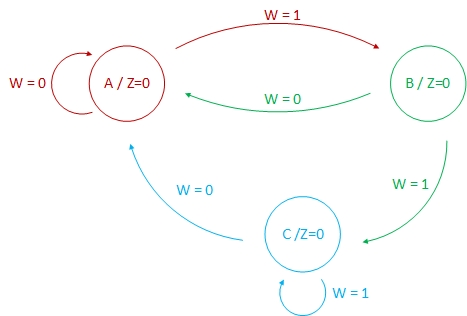
\includegraphics[width=8cm]{Imagenes/mooreej3.jpg}
	\caption{Diagrama Moore }
\end{figure}


%%	TABLA DE TRANSICIONES

\begin{figure}[hbtp]
	\begin{center}
		\begin{tabular}{|c|c|c|c|}
\hline
\multirow{2}{*}{\textbf{ESTADO ACTUAL}} & \multicolumn{2}{c|}{\textbf{ESTADO SIGUIENTE}} & \textbf{SALIDA} \\ \cline{2-4} 
 & \textbf{W=0} & \textbf{W=1} & \textbf{Z} \\ \hline
\textbf{A} & \textbf{A} & \textbf{B} & \textbf{0} \\ \hline
\textbf{B} & \textbf{A} & \textbf{C} & \textbf{1} \\ \hline
\textbf{C} & \textbf{A} & \textbf{C} & \textbf{0} \\ \hline
\textbf{D} & \textbf{X} & \textbf{X} & \textbf{X} \\ \hline
		\end{tabular}
		\caption{Transiciones de Estados - Máquina de Moore} 
		\label{3_fig1}
	\end{center}
\end{figure}


%	TRANSICIONES CON FLIP FLOP
\begin{figure}[hbtp]
	\begin{center}
		\begin{tabular}{|c|c|c|c|c|c|c|}
\hline
\multicolumn{2}{|c|}{\multirow{2}{*}{\textbf{ESTADO ACTUAL}}} & \multicolumn{4}{c|}{\textbf{ESTADO SIGUIENTE}} & \multirow{2}{*}{\textbf{SALIDA}} \\ \cline{3-6}
\multicolumn{2}{|c|}{} & \multicolumn{2}{c|}{\textbf{W = 0}} & \multicolumn{2}{c|}{\textbf{W = 1}} &  \\ \hline
\textbf{$Q_{1_{t}}$} & \textbf{$Q_{0_{t}}$} & \textbf{$Q_{1_{t+1}}$} & \textbf{$Q_{0_{t+1}}$} & \textbf{$Q_{1_{t+1}}$} & \textbf{$Q_{0_{t}}$} & \textbf{Z} \\ \hline
\textbf{0} & \textbf{0} & \textbf{0} & \textbf{0} & \textbf{0} & \textbf{1} & \textbf{0} \\ \hline
\textbf{0} & \textbf{1} & \textbf{0} & \textbf{0} & \textbf{1} & \textbf{0} & \textbf{1} \\ \hline
\textbf{1} & \textbf{0} & \textbf{0} & \textbf{0} & \textbf{1} & \textbf{0} & \textbf{0} \\ \hline
\textbf{1} & \textbf{1} & \textbf{X} & \textbf{X} & \textbf{X} & \textbf{X} & \textbf{X} \\ \hline
		\end{tabular}
		\caption{Transiciones con Flip Flop - Máquina de Moore} 
		\label{3_fig2}
	\end{center}
\end{figure}


%	MAPA Karnaugh Q0
\begin{figure}[H]
	\begin{center}
		\begin{KarnaughvuiteTP3}
		\minterms{4}
		\maxterms{0,1,2,5,6}
		\indeterminats{3,7}
		\implicant{4}{4}{orange}
		\end{KarnaughvuiteTP3}
	\end{center}
	\caption{$Q_0$: Máq. de Moore} 
	\label{3_fig3}
\end{figure}

%	MAPA Karnaugh Q1
\begin{figure}[H]
	\begin{center}
		\begin{KarnaughvuiteTP3}
		\minterms{5,6}
		\maxterms{0,1,2,4}
		\indeterminats{3,7}
		\implicant{5}{7}{orange}
		\implicant{7}{6}{blue}
		\end{KarnaughvuiteTP3}
	\end{center}
	\caption{$Q_1$ Máq. de Moore} 
	\label{3_fig4}
\end{figure}

%	MAPA Karnaugh Z
\begin{figure}[H]
	\begin{center}
		\begin{KarnaughquatreTP3}
		\minterms{1}
		\maxterms{0,2}
		\indeterminats{3}
		\implicantsol{1}{green}
		\end{KarnaughquatreTP3}
	\end{center}
	\caption{$Z$: Máq. de Moore} 
	\label{3_fig5}
\end{figure}



%% EXPLICACION DEL ANALISIS
Al reducir los minitérminos obtuvimos las siguientes expresiones que representan el circuito lógico que se usara para resolver la máquina de estado:

\begin{align*}
	Q_{0_{t+1}} &= W * \overline{Q_{1}} * \overline{Q_{0}}\\
	Q_{1_{t+1}} &= W * (Q_{1} + Q_{0})  \\
	Z &= Q_{0} \\
\end{align*}


Entonces el circuito quedará de la siguiente manera:

\begin{figure}[H]
	\centering
	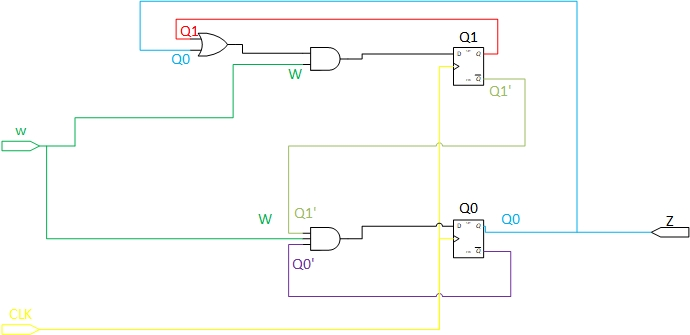
\includegraphics[width=8cm]{Imagenes/circej3moore.jpg}
	\caption{Circuito lógico - Moore}
	\label{3_fig6}
\end{figure}


\subsection*{Mealy}
Analizando las tablas de transiciones de estados pudimos notar que la función de la máquina es prender la salida cuando se recibe la primer señal en HIGH y luego se apaga en el segundo CLOCK. Para implementar ahora la máquina de Mealy tuvimos en cuenta esto y diseñamos el siguiente diagrama.

%% DIAGRAMA DE MEALY
\begin{figure}[hbtp]
	\centering
	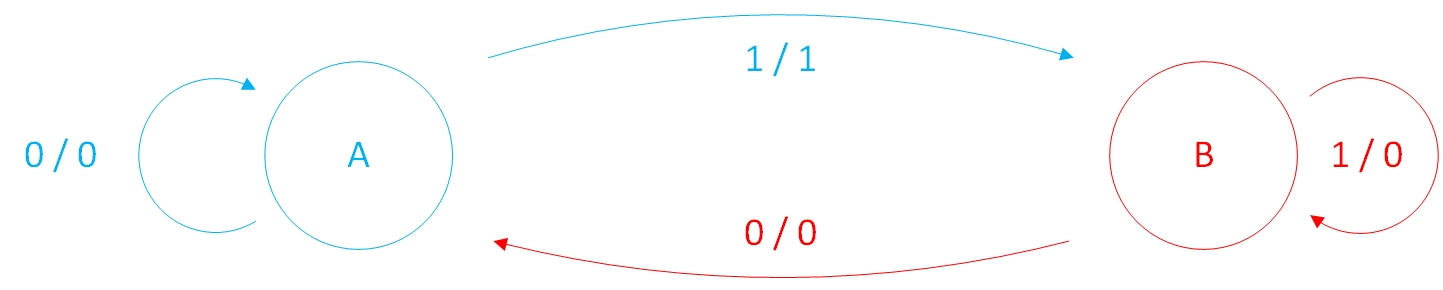
\includegraphics[width=8cm]{Imagenes/mealyej3.jpg}
	\caption{Diagrama de Mealy}
\end{figure}

De este diagrama representamos en una tabla la transiciones de estados directamente con un Flip Flop, ya que al haber solo 2 estados solo se necesita un Flip Flop para representar ambos estados, el estado 0 y estado 1. La tabla es la siguiente:

\begin{figure}[H]
	\begin{center}
		\begin{tabular}{|c|c|c|c|c|}
\hline
\multirow{2}{*}{\textbf{ESTADO ACTUAL}} & \multicolumn{2}{c|}{\textbf{ESTADO SIGUIENTE}} & \multicolumn{2}{c|}{\textbf{SALIDA}} \\ \cline{2-5} 
 & \multicolumn{2}{c|}{\textbf{Q}} & \multicolumn{2}{c|}{\textbf{Z}} \\ \hline
\textbf{Q} & \textbf{W=0} & \textbf{W=1} & \textbf{W=0} & \textbf{W=1} \\ \hline
\textbf{0} & \textbf{0} & \textbf{1} & \textbf{0} & \textbf{1} \\ \hline
\textbf{1} & \textbf{0} & \textbf{1} & \textbf{0} & \textbf{0} \\ \hline
		\end{tabular}
		\caption{Transiciones con Flip Flop - Máquina de Moore} 
		\label{3_fig8}
	\end{center}
\end{figure}

Sin un análisis muy complejo, el flip flop devuelve una salida en HIGH solo cuando la entrada es HIGH, e igualmente cuando devuelven una señal LOW, por lo que la salida será directamente la entrada. Pero la salida depende tanto del estado como de la entrada, característica de este tipo de máquina de estado, por lo que la salida será:

\begin{align*}
	Z &= W * \overline{Q_{0}} \\
\end{align*}
El circuito lógico queda muy simple a comparación del logrado con Moore, demostrado en la siguiente figura:

\begin{figure}[H]
	\centering
	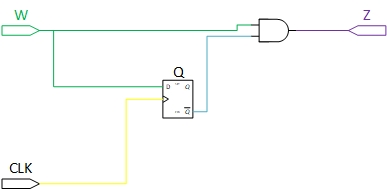
\includegraphics[width=8cm]{Imagenes/circej3mealy.jpg}
	\caption{Circuito lógico Mealy}
\end{figure}


\subsection*{Implementación}
Para crear ambas máquinas se pidió que las entradas y salidas del circuito deberán ser lógica de 5V, mientras que toda la lógica interna trabajará con 3,3V. Para esto hicimos un circuito que pueda bajar de 5V a 3,3V y viceversa. Este circuito puede verse abajo, en donde LI es la tensión con la que trabajamos (3,3V o 5V dependiendo el caso), HV es la tensión de alimentación (de nuevo 3,3V o 5V pero sin ser igual a LI) y HO la salida que va a tener la tensión deseada. Cuando LI sea sea interpretada como estado alto, HO será 5V si LI es 3.3V y HV 5V, en caso de ser LI 5V y HV 3,3V, HO será 3,3V. Si LI es interpretada como estado bajo, HO será 0V.

\begin{figure}[H]
	\centering
	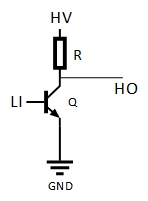
\includegraphics[scale=1]{Imagenes/Conversor.jpg}
	\caption{Conversor}
\end{figure}

Observamos que las tecnologías TTL y CMOS aceptaban bien los valores de 3,3V como señal HIGH para estos circuitos, por lo que no tuvimos restricción con respecto a las tecnologías.
En la siguiente imagen se puede ver como la salida cambia cuando el clock es HIGH y la entrada también, pero al segundo CLOCK se apaga aunque la entrada siga en HIGH, demostrando que solo se prende con el primer 1 lógico recibido.
\begin{figure}[H]
	\centering
	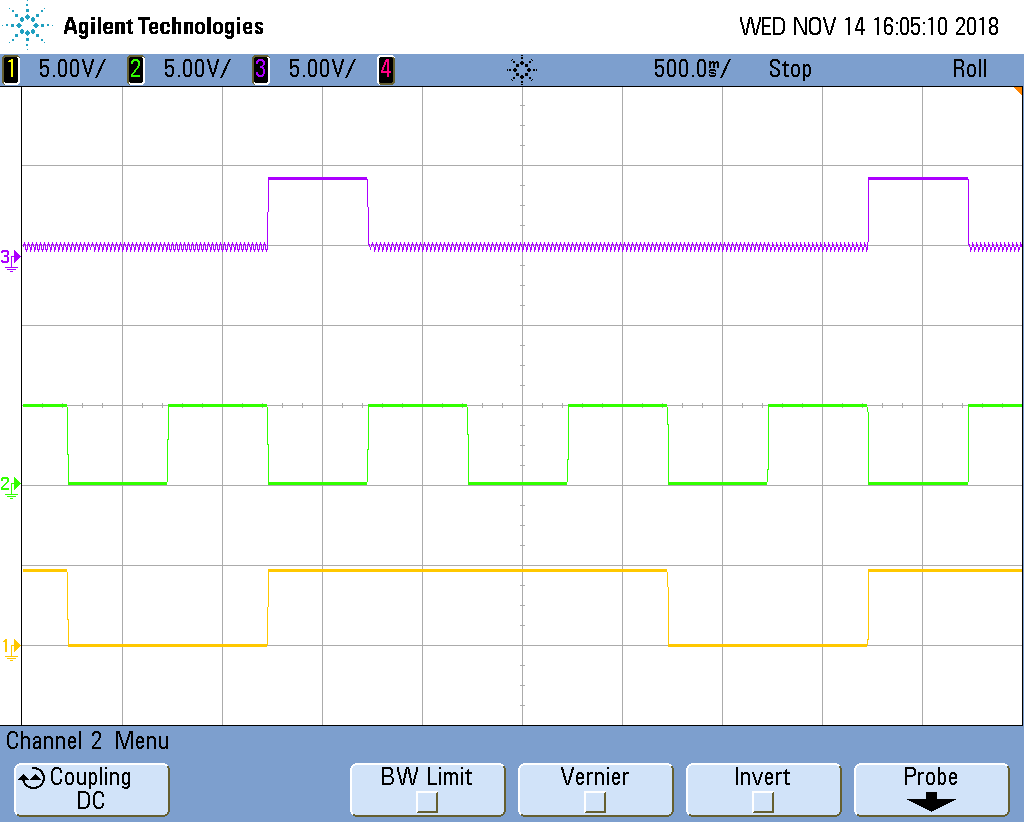
\includegraphics[width=14cm]{Imagenes/MedicionTP3_Ej3.png}
	\caption{Medición del Ejercicio 3}
\end{figure}

\subsection*{Conclusión}
Pudimos observar el buen funcionamiento de ambas máquinas cumpliendo la misma función, aunque el circuito resuelto con Mealy necesito solo 2 componentes (que serían 2 integrados) por lo que resulta más simple y económico, también tiene menos delay la salida ya que solo consta de una compuerta.


\end{document}